
\documentclass[11pt]{article}


\usepackage{fullpage}
\usepackage{amsmath}
\usepackage{amssymb}
\usepackage{algorithm}
\usepackage{algpseudocode}

\usepackage{verbatim}

\usepackage[scr=boondoxo]{mathalfa}

\usepackage{graphicx}
\usepackage{xcolor}

\usepackage{pdfpages}

\usepackage[round]{natbib}

\newcommand{\N}{\mathcal{N}}
\newcommand{\A}{\mathcal{A}}
\newcommand{\Z}{\mathcal{Z}}
\newcommand{\tff}{t^{\mathrm{ff}}_{ij}}


\usepackage[colorlinks=true]{hyperref}
\hypersetup{%
	urlcolor=blue,% hyperlink text will be green
	linkcolor=black,
	citecolor=black,
	filecolor=black
}


\DeclareMathOperator*{\argmin}{\arg\min}



\begin{document}
	\allowdisplaybreaks[1]
	
	
	\title{A tutorial for programming static traffic assignment in Python}
	
	\author{Michael W. Levin}
	
	\maketitle
	
\section{Introduction}

The purpose of this tutorial is to guide you through learning the programming concepts necessary to implement the method of successive averages for solving user equilibrium. (For more information on user equilibrium, see \href{https://sboyles.github.io/blubook.html}{\textit{Transportation Network Analysis}}.)
This tutorial consists of a series of programming exercises that increase in difficulty and required programming knowledge. After completing all exercises, you will have a working implementation of the method of successive averages. 
To assist with these exercises, I have linked relevant programming tutorials and provided an autograde to check correctness. Some code is provided as a starting point. 
This tutorial and the code is based on the Python programming language and object-oriented programming.
%
%For your convenience, printed versions of all external tutorial pages referenced here have been included at the end of this document. 


\subsection{Getting started}
\label{sec11}

The existing code is provided as a Netbeans project. You may use Netbeans or an alternative of your choice.
\paragraph*{To use Netbeans:} Download and install \href{https://netbeans.apache.org/download/index.html}{Netbeans}. Follow the \href{https://plugins.netbeans.apache.org/catalogue/?id=89}{instructions here} to install the Python plugin. You may need \href{https://netbeans.apache.org/download/nb18/}{Netbeans version 18} for the plugin to work.

 Download a copy of this Git repository:

\noindent \href{https://github.com/mwlevin/STApractice_python.git}{https://github.com/mwlevin/STApractice\_python.git}. Alternatively, you can \href{https://netbeans.org/kb/docs/ide/git.html#clone}{clone it in Netbeans}.


The repository contains a Netbeans project, which you may open directly in Netbeans. You can also open the source files in another IDE. All source files are in the ``src'' folder, with the exception of main.py. Test data is in the ``data'' folder:

\begin{center}
	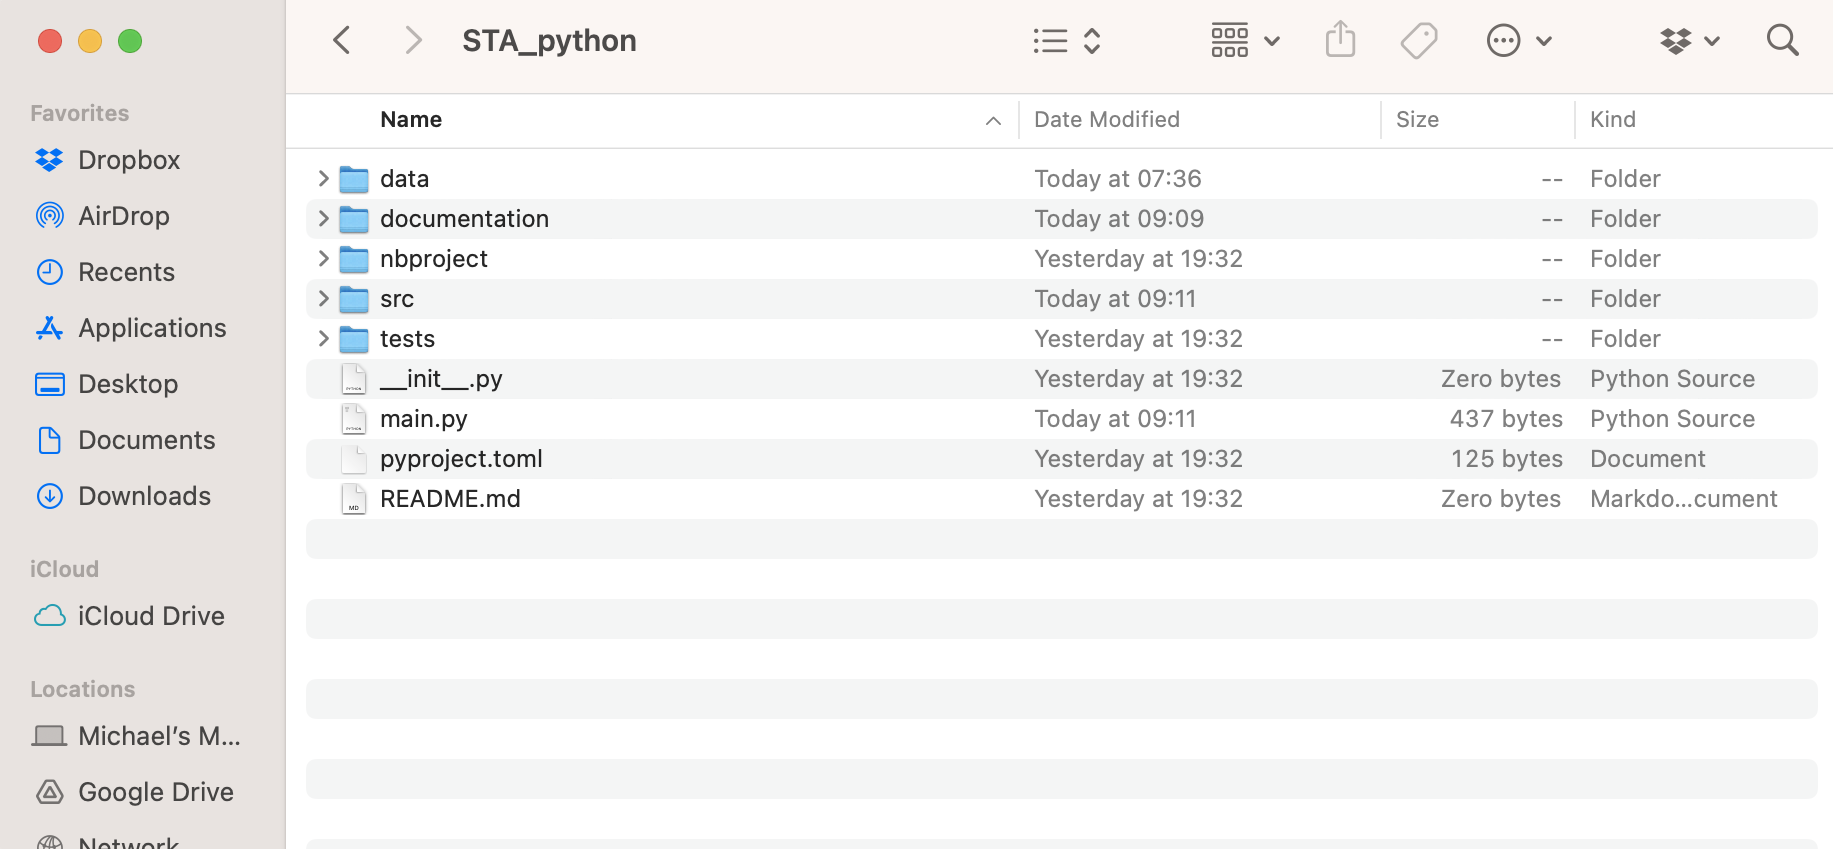
\includegraphics[width=0.7\textwidth]{folder.png}
\end{center}

The \texttt{main()} function (which is executed when you run the program) is found in main.py. Each of the exercises in this tutorial are contained within a separate file, e.g. Exercise1.py, Exercise2.py, etc. Each of these files has their own \texttt{test()} function that can be executed.
In main.py, you will find calls to these functions \href{https://www.w3schools.com/python/python_comments.asp}{commented out}, i.e. \texttt{\#Exercise1.test()}. Uncomment them to run each exercise. 

\begin{center}
	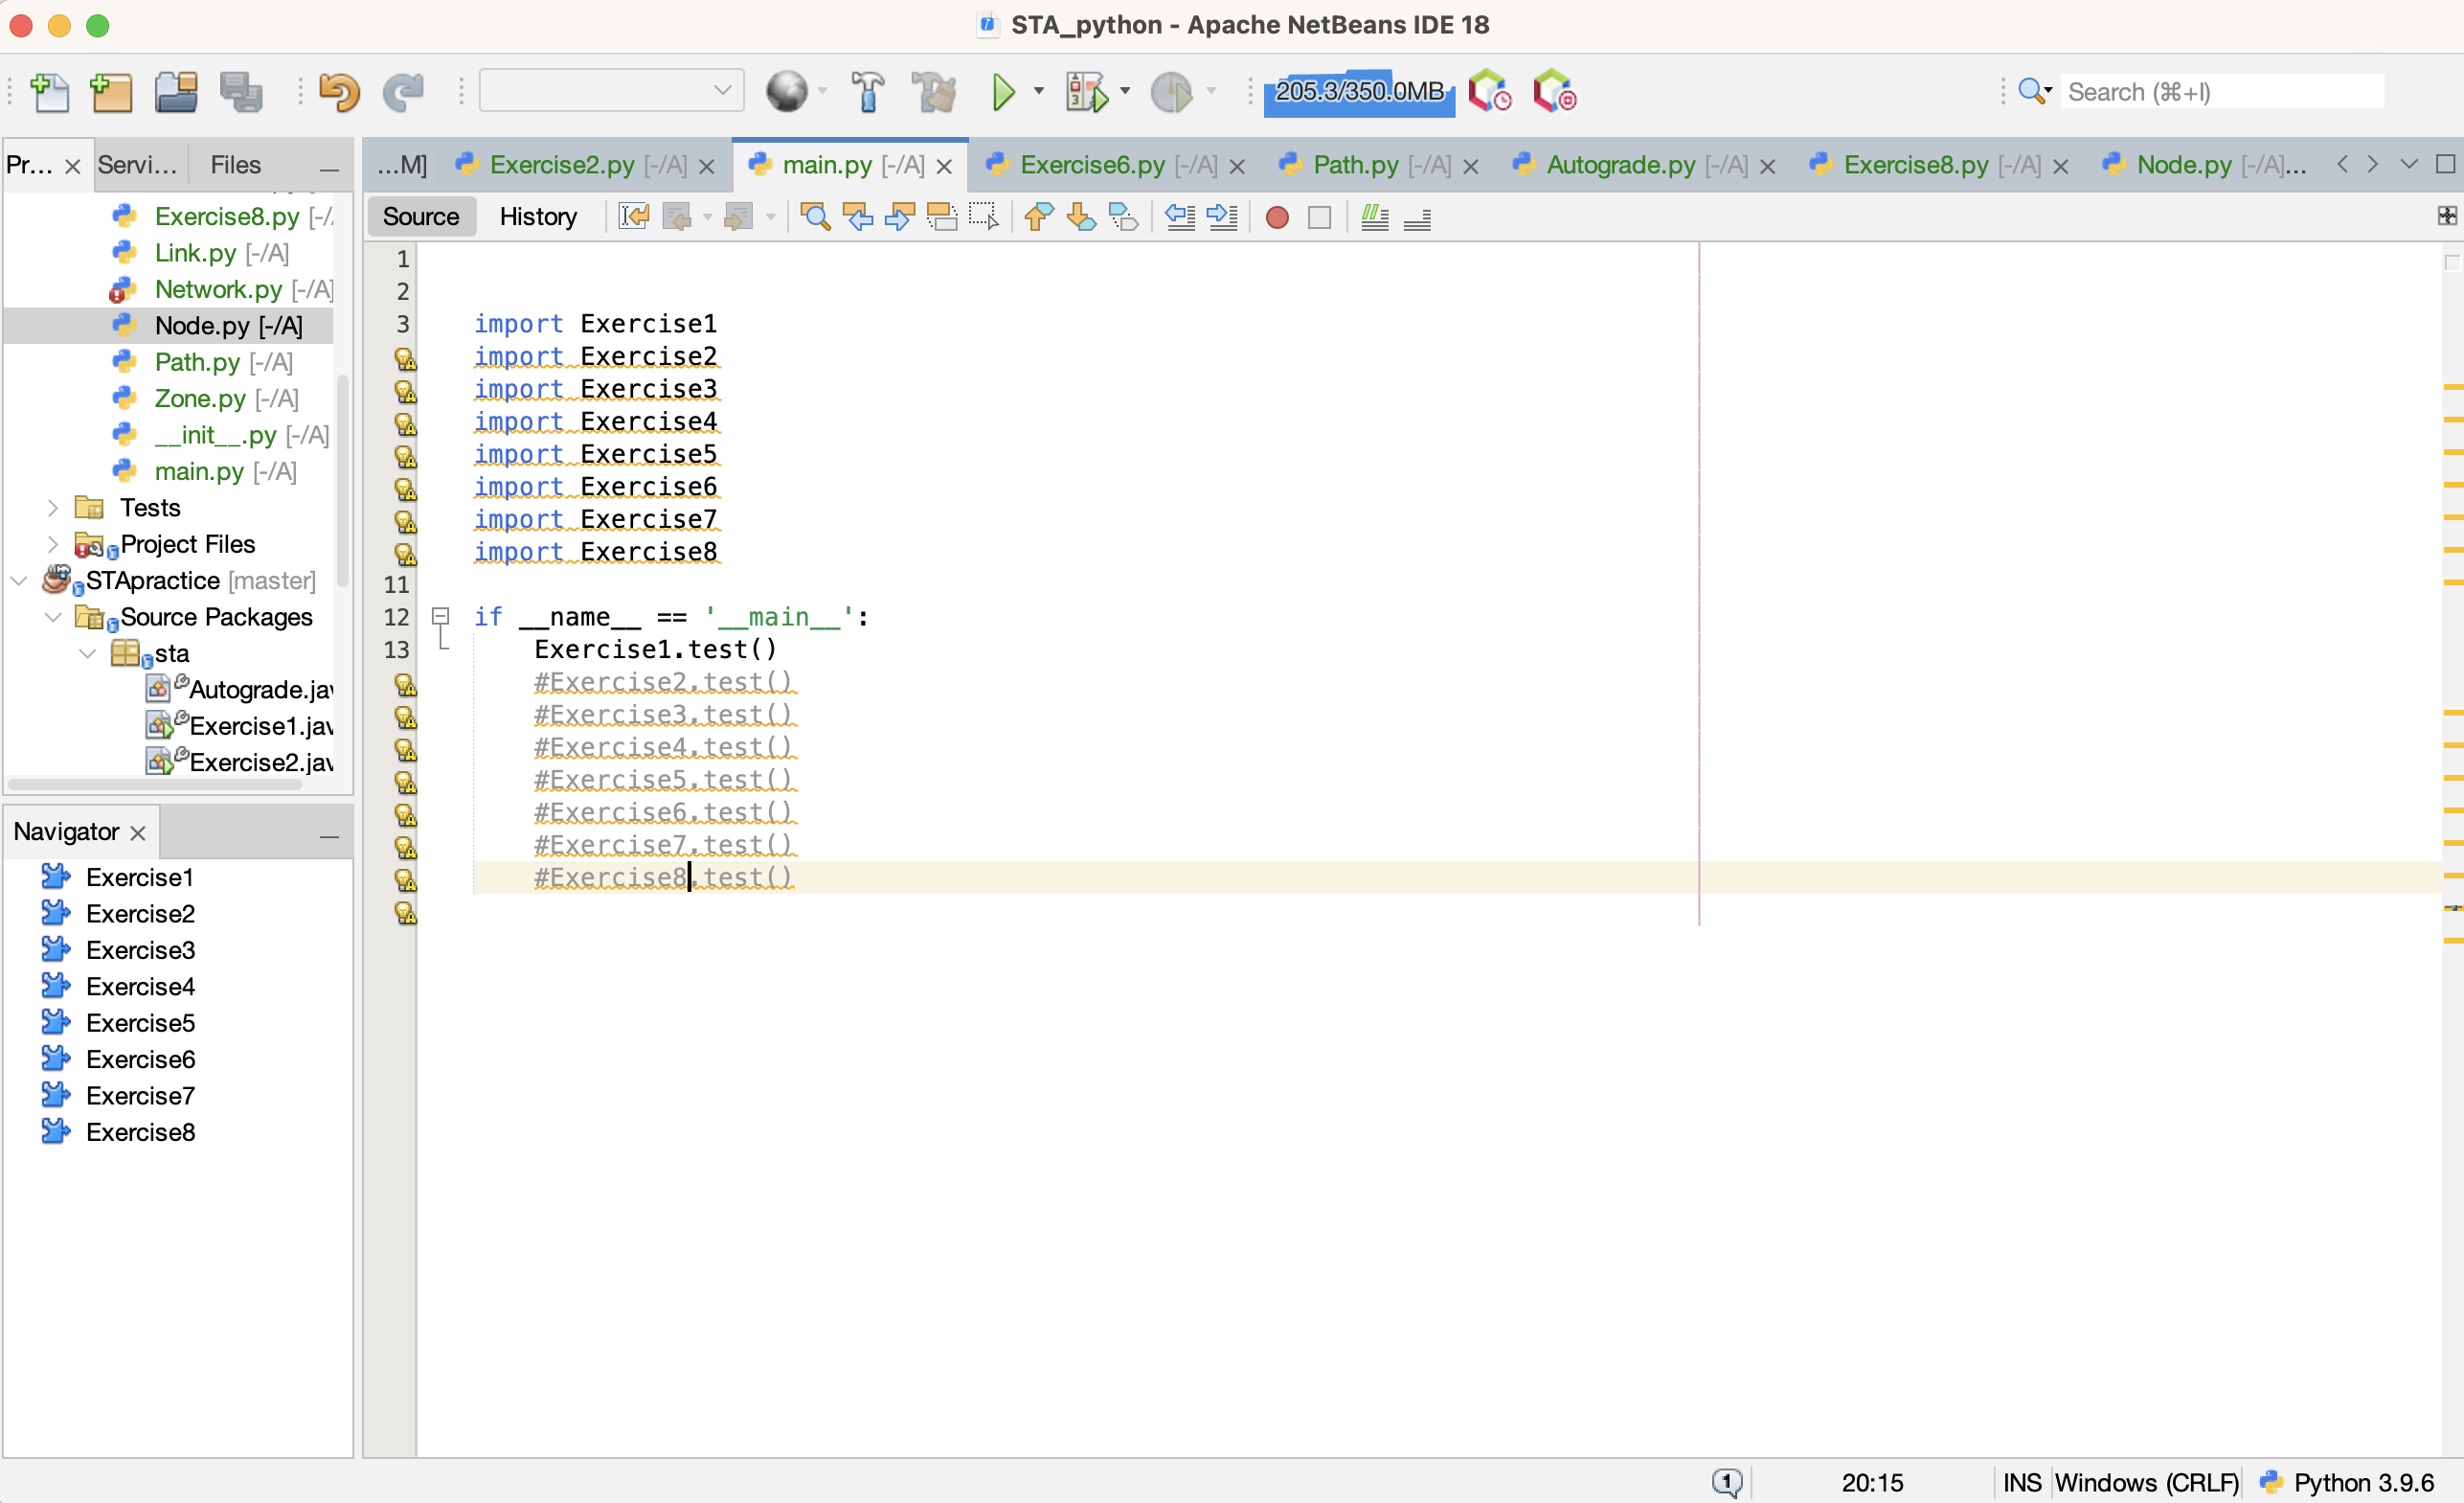
\includegraphics[width=\textwidth]{netbeans1.png}
\end{center}



Each exercise contains some test code. At the end of the \texttt{test()} function, it calls the \texttt{autograde()} function which will automatically test the output of your code against the correct answers. Go ahead and run the code; it should run successfully, but the autograde will indicate that your code is incorrect:

\begin{center}
	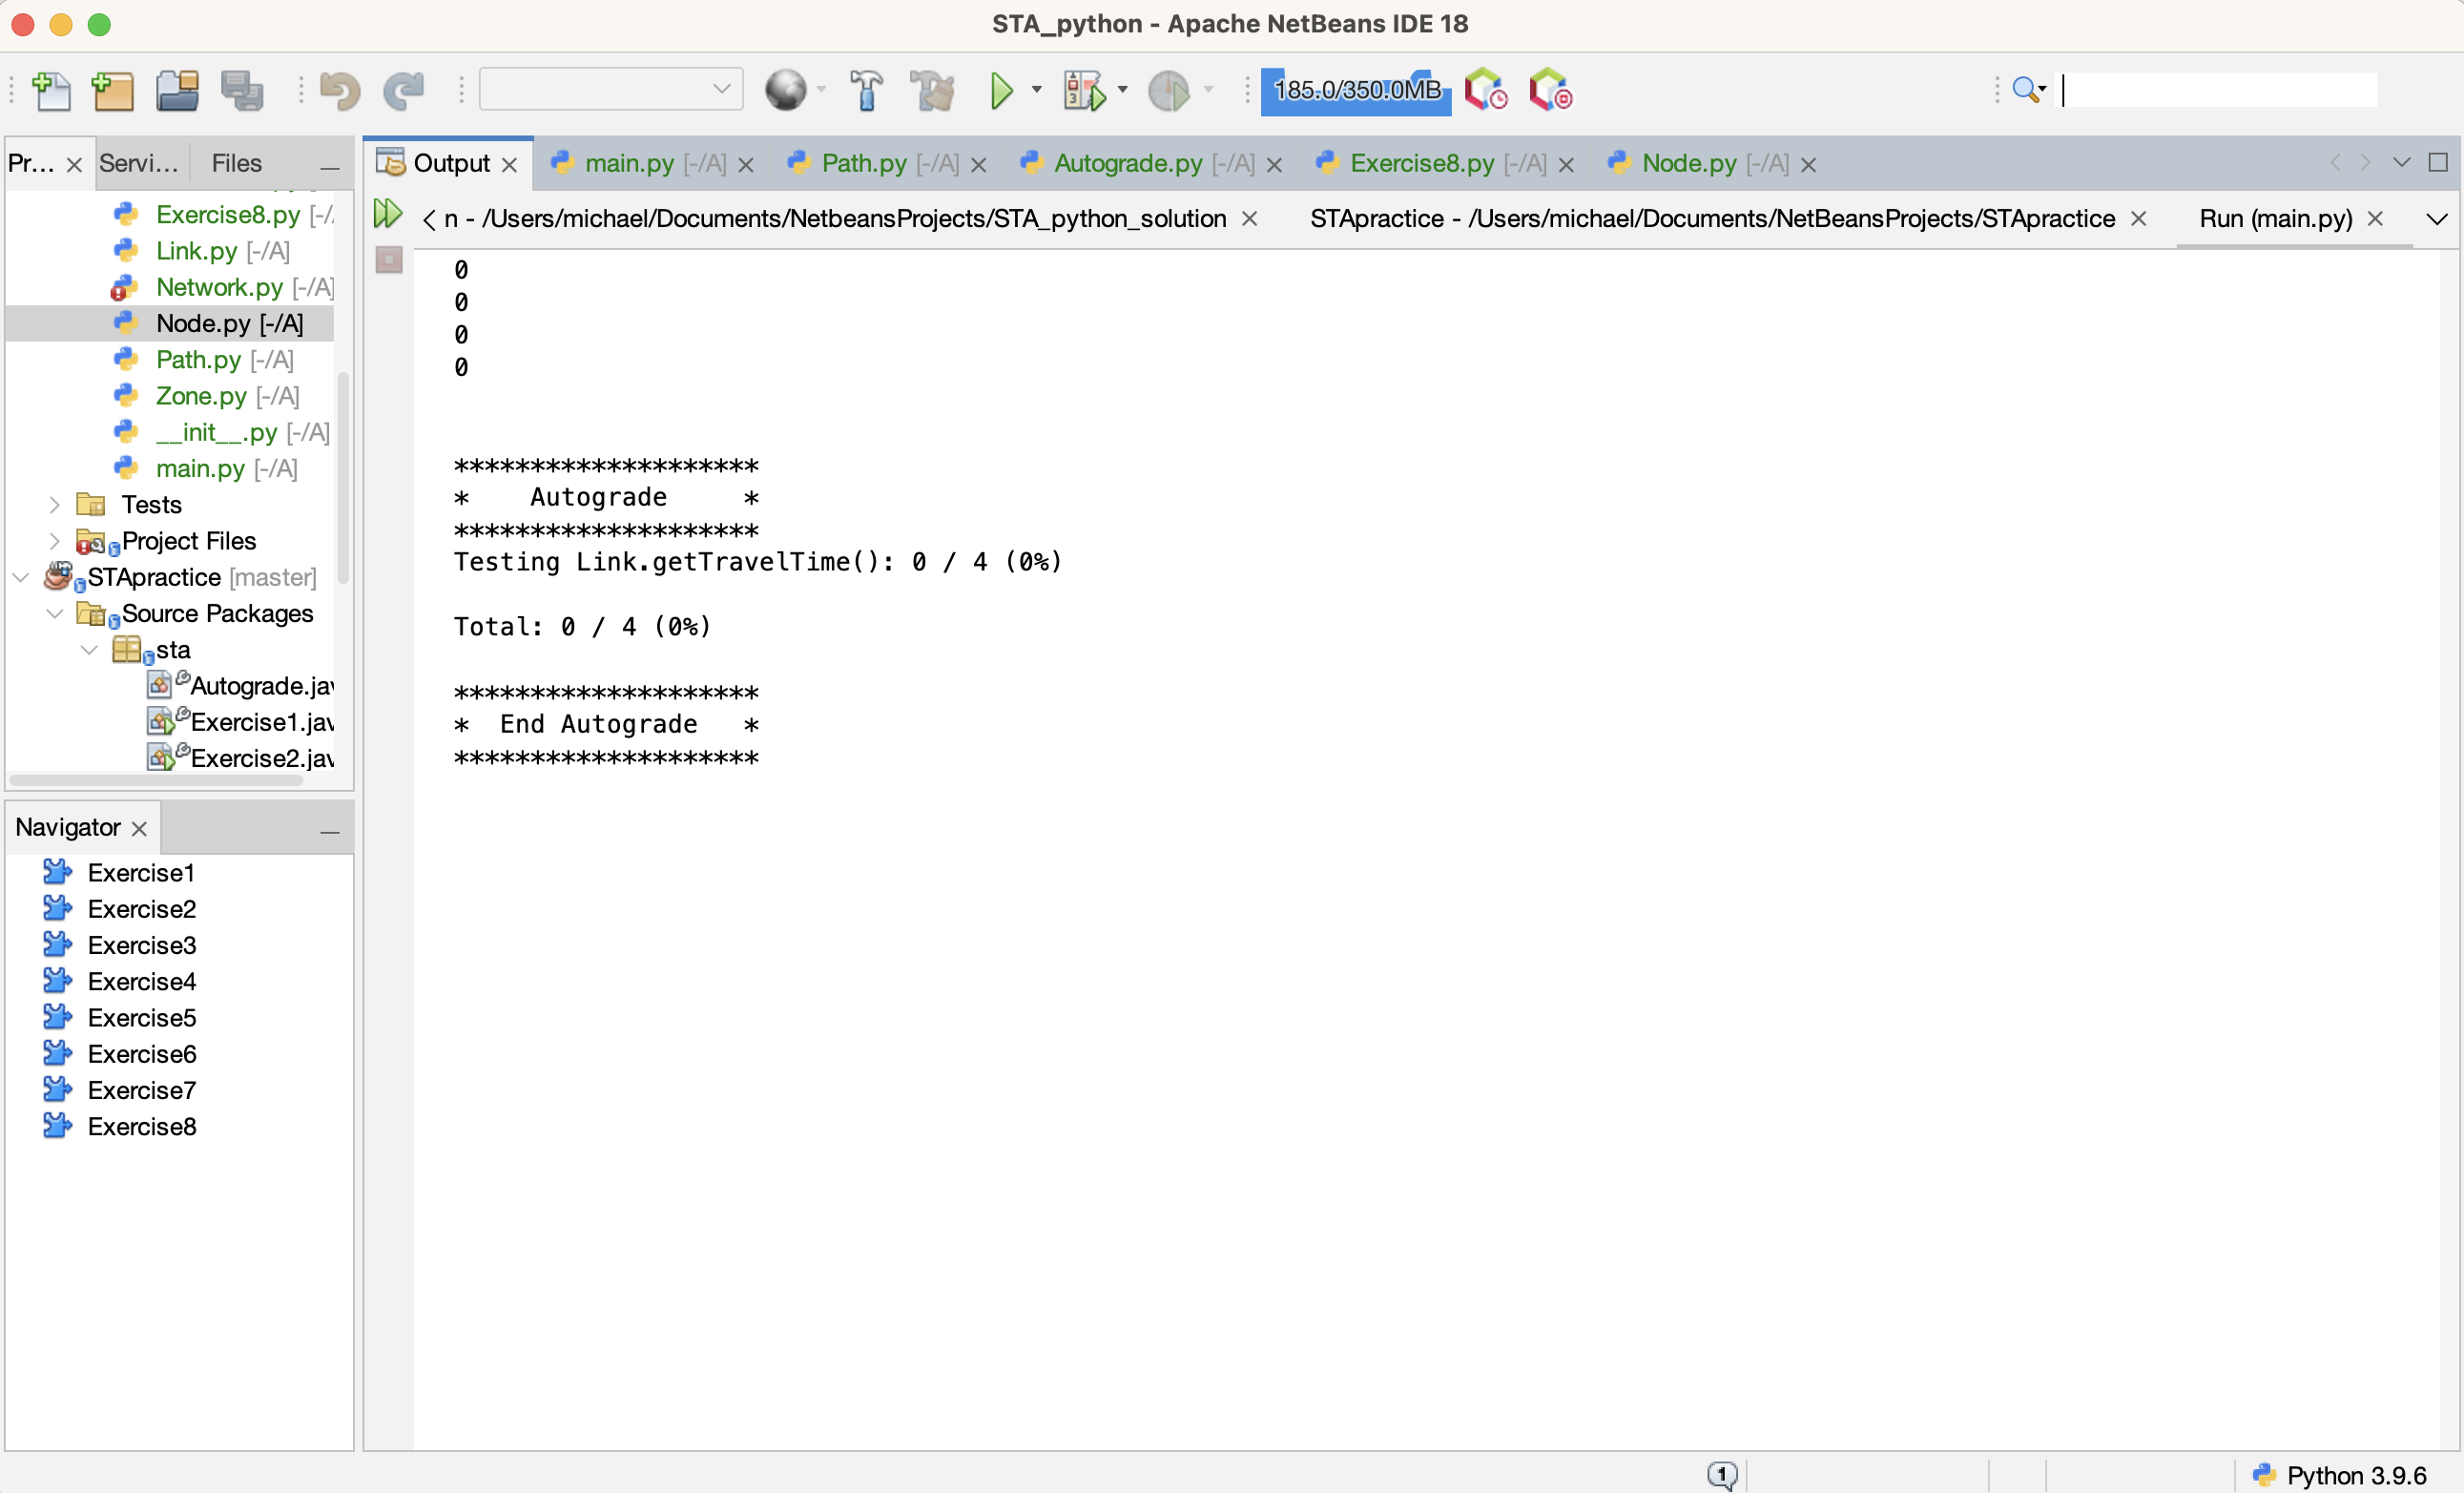
\includegraphics[width=\textwidth]{netbeans1a.png}
\end{center}








\subsection{Notation}

This section defines the notation for the traffic assignment problem being solved. 
For more details on the definition, see \href{https://sboyles.github.io/blubook.html}{\textit{Transportation Network Analysis}}. 
Consider a network $\mathcal{G}=(\N,\A)$ with nodes $\N$ and links $\A\subseteq \N^2$.  Let $\Gamma^+_i\subseteq\A$ be the set of links outgoing from node $i$. The travel time $t_{ij}$ for link $(i,j)\in\A$ is a function of the flow on that link $x_{ij}$, and is given by the BPR function
\begin{equation}
	t_{ij}(x_{ij}) = \tff \left(1+\alpha_{ij} \left(\frac{x_{ij}}{C_{ij}}\right)^{\beta_{ij}}\right) \label{bpr}
\end{equation}
where $\tff$ is the free flow travel time, $C_{ij}$ is the link capacity, and $\alpha_{ij}$ and $\beta_{ij}$ are calibration constants.


Let $\Z\subseteq\N$ be the set of zones. All trips start and end at zones. The demand from zone $r$ to zone $s$ is denoted as $d_{rs}$. A path $\pi$ consists of a set of links. Let $\Pi$ be the set of all paths, and let $\Pi_{rs}\subseteq\Pi$ be the set of paths from $r$ to $s$. Let $h^\pi$ be the flow on path $\pi$, and let $T^\pi$ be the travel time for path $\pi$. Let $\delta^\pi_{ij}\in\{0,1\}$ indicate whether path $\pi$ includes link $(i,j)$. Then $T^\pi$ can be written as
\begin{equation}
	T^\pi = \sum\limits_{(i,j)\in\A} \delta^\pi_{ij} t_{ij}(x_{ij})
\end{equation}
The user equilibrium problem is to find a path flow assignment $\mathbf{h}$ such that
\begin{align}
	h^\pi \left(T^\pi - \mu_{rs}\right) = 0
\end{align}
where $\mu_{rs}$ is the minimum travel time from $r$ to $s$. The solution can be found by solving the convex program
\begin{subequations}
\begin{align}
	& \min && Z=\sum\limits_{(i,j)\in\A} \int\limits_{0}^{x_{ij}} t_{ij}(\omega) d\omega && \\
	& \mathrm{s.t.} && x_{ij} = \sum\limits_{\pi \in \Pi} \delta^\pi_{ij} h^\pi && \forall (i,j)\in\A\\
	& && d_{rs} = \sum\limits_{\pi\in\Pi_{rs}} h^\pi && \forall (r,s)\in\Z^2\\
	& && h^\pi \geq 0 && \forall \pi\in\Pi 
\end{align}
\end{subequations}
This tutorial will guide you through the steps needed to implement the method of successive averages algorithm for solving this problem.






\section{Primitive data types, control logic, and arrays}

\subsection{Calculating link travel times}
\label{sec21}

First, review \href{https://www.w3schools.com/python/python_syntax.asp}{Python syntax} and \href{https://www.w3schools.com/python/python_comments.asp}{comments}.
Read the tutorials on \href{https://www.w3schools.com/python/python_variables.asp}{variables} and \href{https://www.w3schools.com/python/python_datatypes.asp}{data types}. 


Open Link.py. You will notice that the code first defines a \texttt{class Link}, which is a new data type intended represent one link $(i,j)\in\A$. Each $(i,j)$ should have a separate instance of the \texttt{Link} class. 
We will learn later about creating and working with classes in Python. You will see some variables \texttt{x}, \texttt{t\_ff}, \texttt{C}, \texttt{alpha}, and \texttt{beta} defined in the function \texttt{\_\_init\_\_()}. For now, it is sufficient to know that these variables are available for use anywhere within the \texttt{Link} class by using the \href{https://www.w3schools.com/python/gloss_python_self.asp}{``\texttt{self}'' reference}. These variables correspond to the model variables $x_{ij}$, $t^{\mathrm{ff}}_{ij}$, $C_{ij}$, $\alpha_{ij}$, and $\beta_{ij}$ for the specific link $(i,j)$ being represented. 

\begin{center}
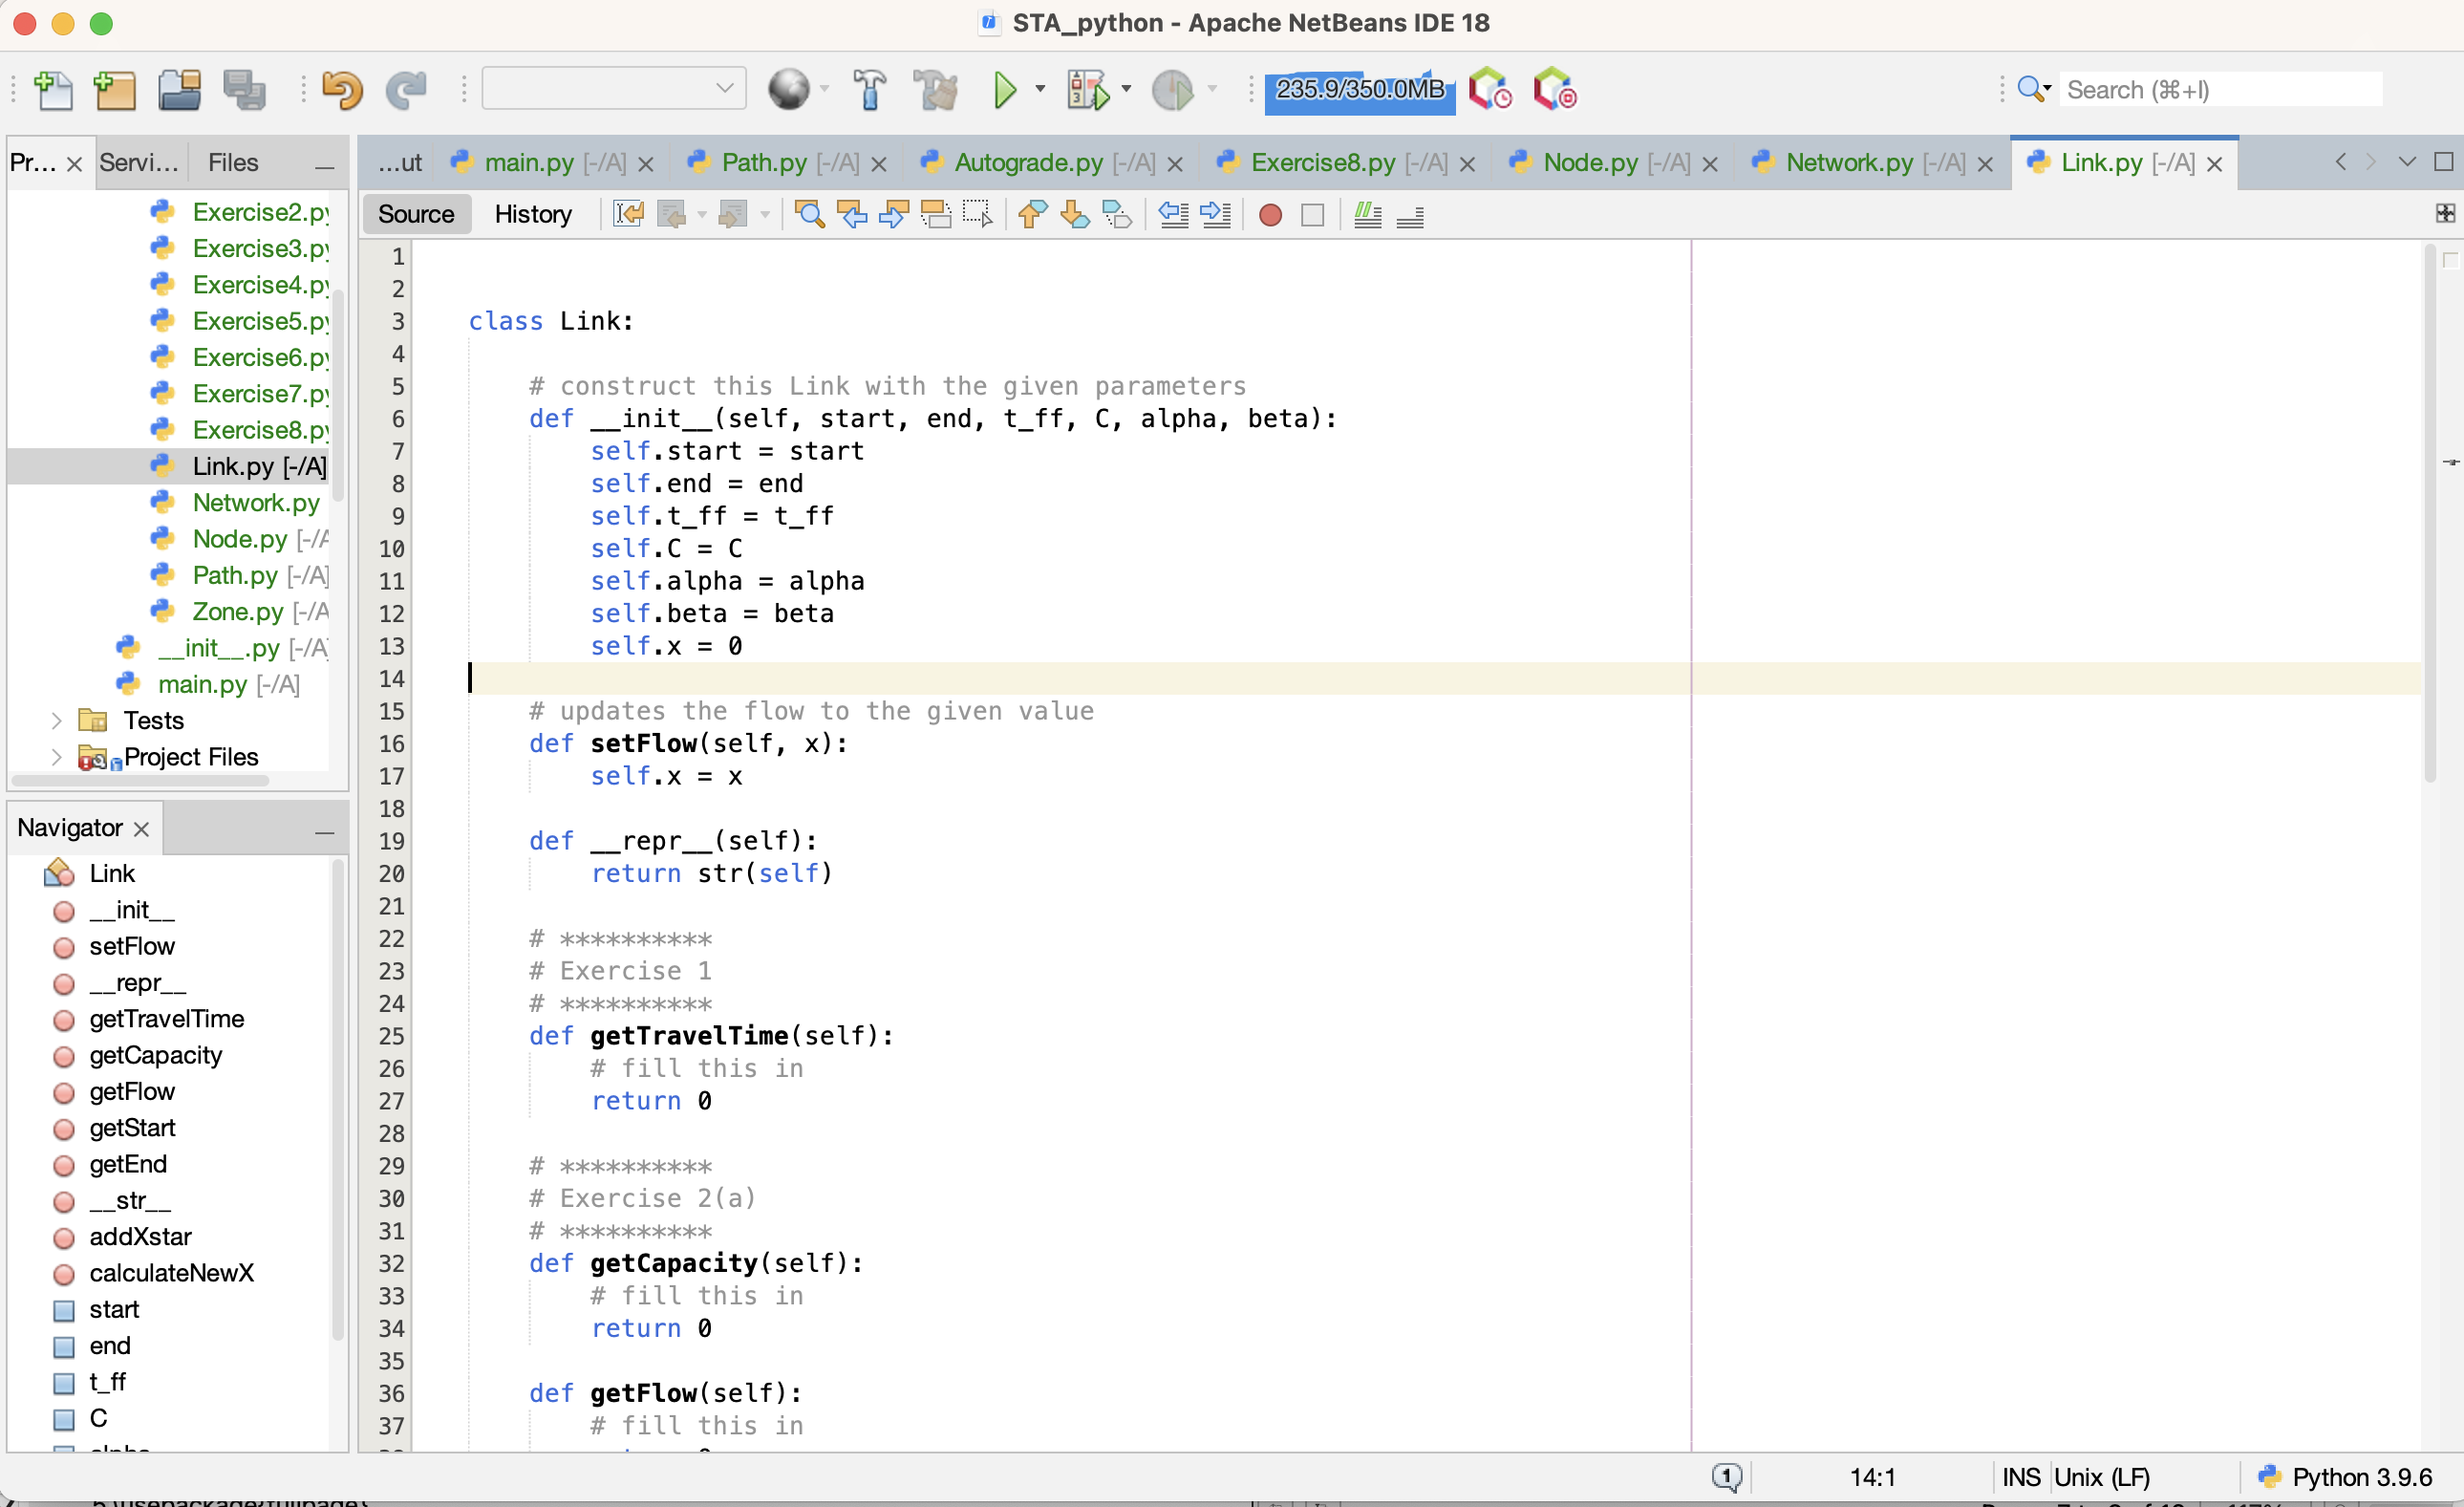
\includegraphics[width=\textwidth]{netbeans2.png}
\end{center}


\noindent Read the  tutorials on \href{https://www.w3schools.com/python/python_operators.asp}{operators} and the \href{https://www.w3schools.com/python/python_math.asp}{math functions}. 
	
	
	The tutorial will list specific exercises of code implementation that are designed to be completed sequentially as they build on the code written previously. The autograde may not be able to check correctness if you complete them out of order. We are now ready for the first exercise.
	
\paragraph*{Exercise 1} Your first task is to implement the calculation of the link travel time $t_{ij}(x_{ij})$ using the BPR function of equation \eqref{bpr}. Assume that the values of $x_{ij}$, $\tff$, $C_{ij}$, $\alpha_{ij}$, and $\beta_{ij}$ are already given. 

Within the \texttt{Link} class in Link.py, find the function labeled \texttt{getTravelTime()}. It defines a variable \texttt{t\_{ij}} and sets the value to 0.0 --- a floating-point number. You need to calculate the correct value of $t_{ij}(x_{ij})$ and assign it to variable \texttt{t\_ij}. 
	
	\begin{center}
		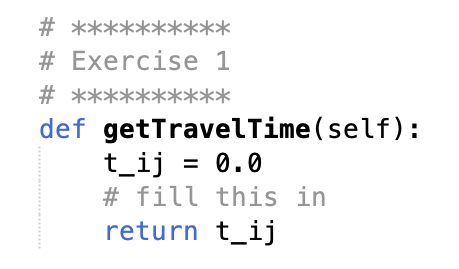
\includegraphics[width=0.3\textwidth]{netbeans3.png}
	\end{center}

\noindent Open main.py and ensure that it will run \texttt{Exercise1.test()}.
Open Exercise1.py. The \texttt{main()} method constructs two instances of the \texttt{Link} class with different parameters. The first link has $t^{\mathrm{ff}}_{1}=10$, $C_{1}=2580$, $\alpha_{1}=0.15$, and $\beta_{1}=4$. The second link $t^{\mathrm{ff}}_{2}=12$, $C_{2}=1900$, $\alpha_{2}=0.35$, and $\beta_{2}=2$. The \texttt{main()} function then prints the calculation of $t_{ij}$ with $x_{1}=1230.2$, $x_2=570$, $x_1=0$, and $x_2=2512$. You should compare the values calculated by your code with values that you have computed by hand. 
Afterwards, \texttt{test()} calls the \texttt{autograde()} function, which runs an automated test of your answers. 
	
	
	\begin{center}
	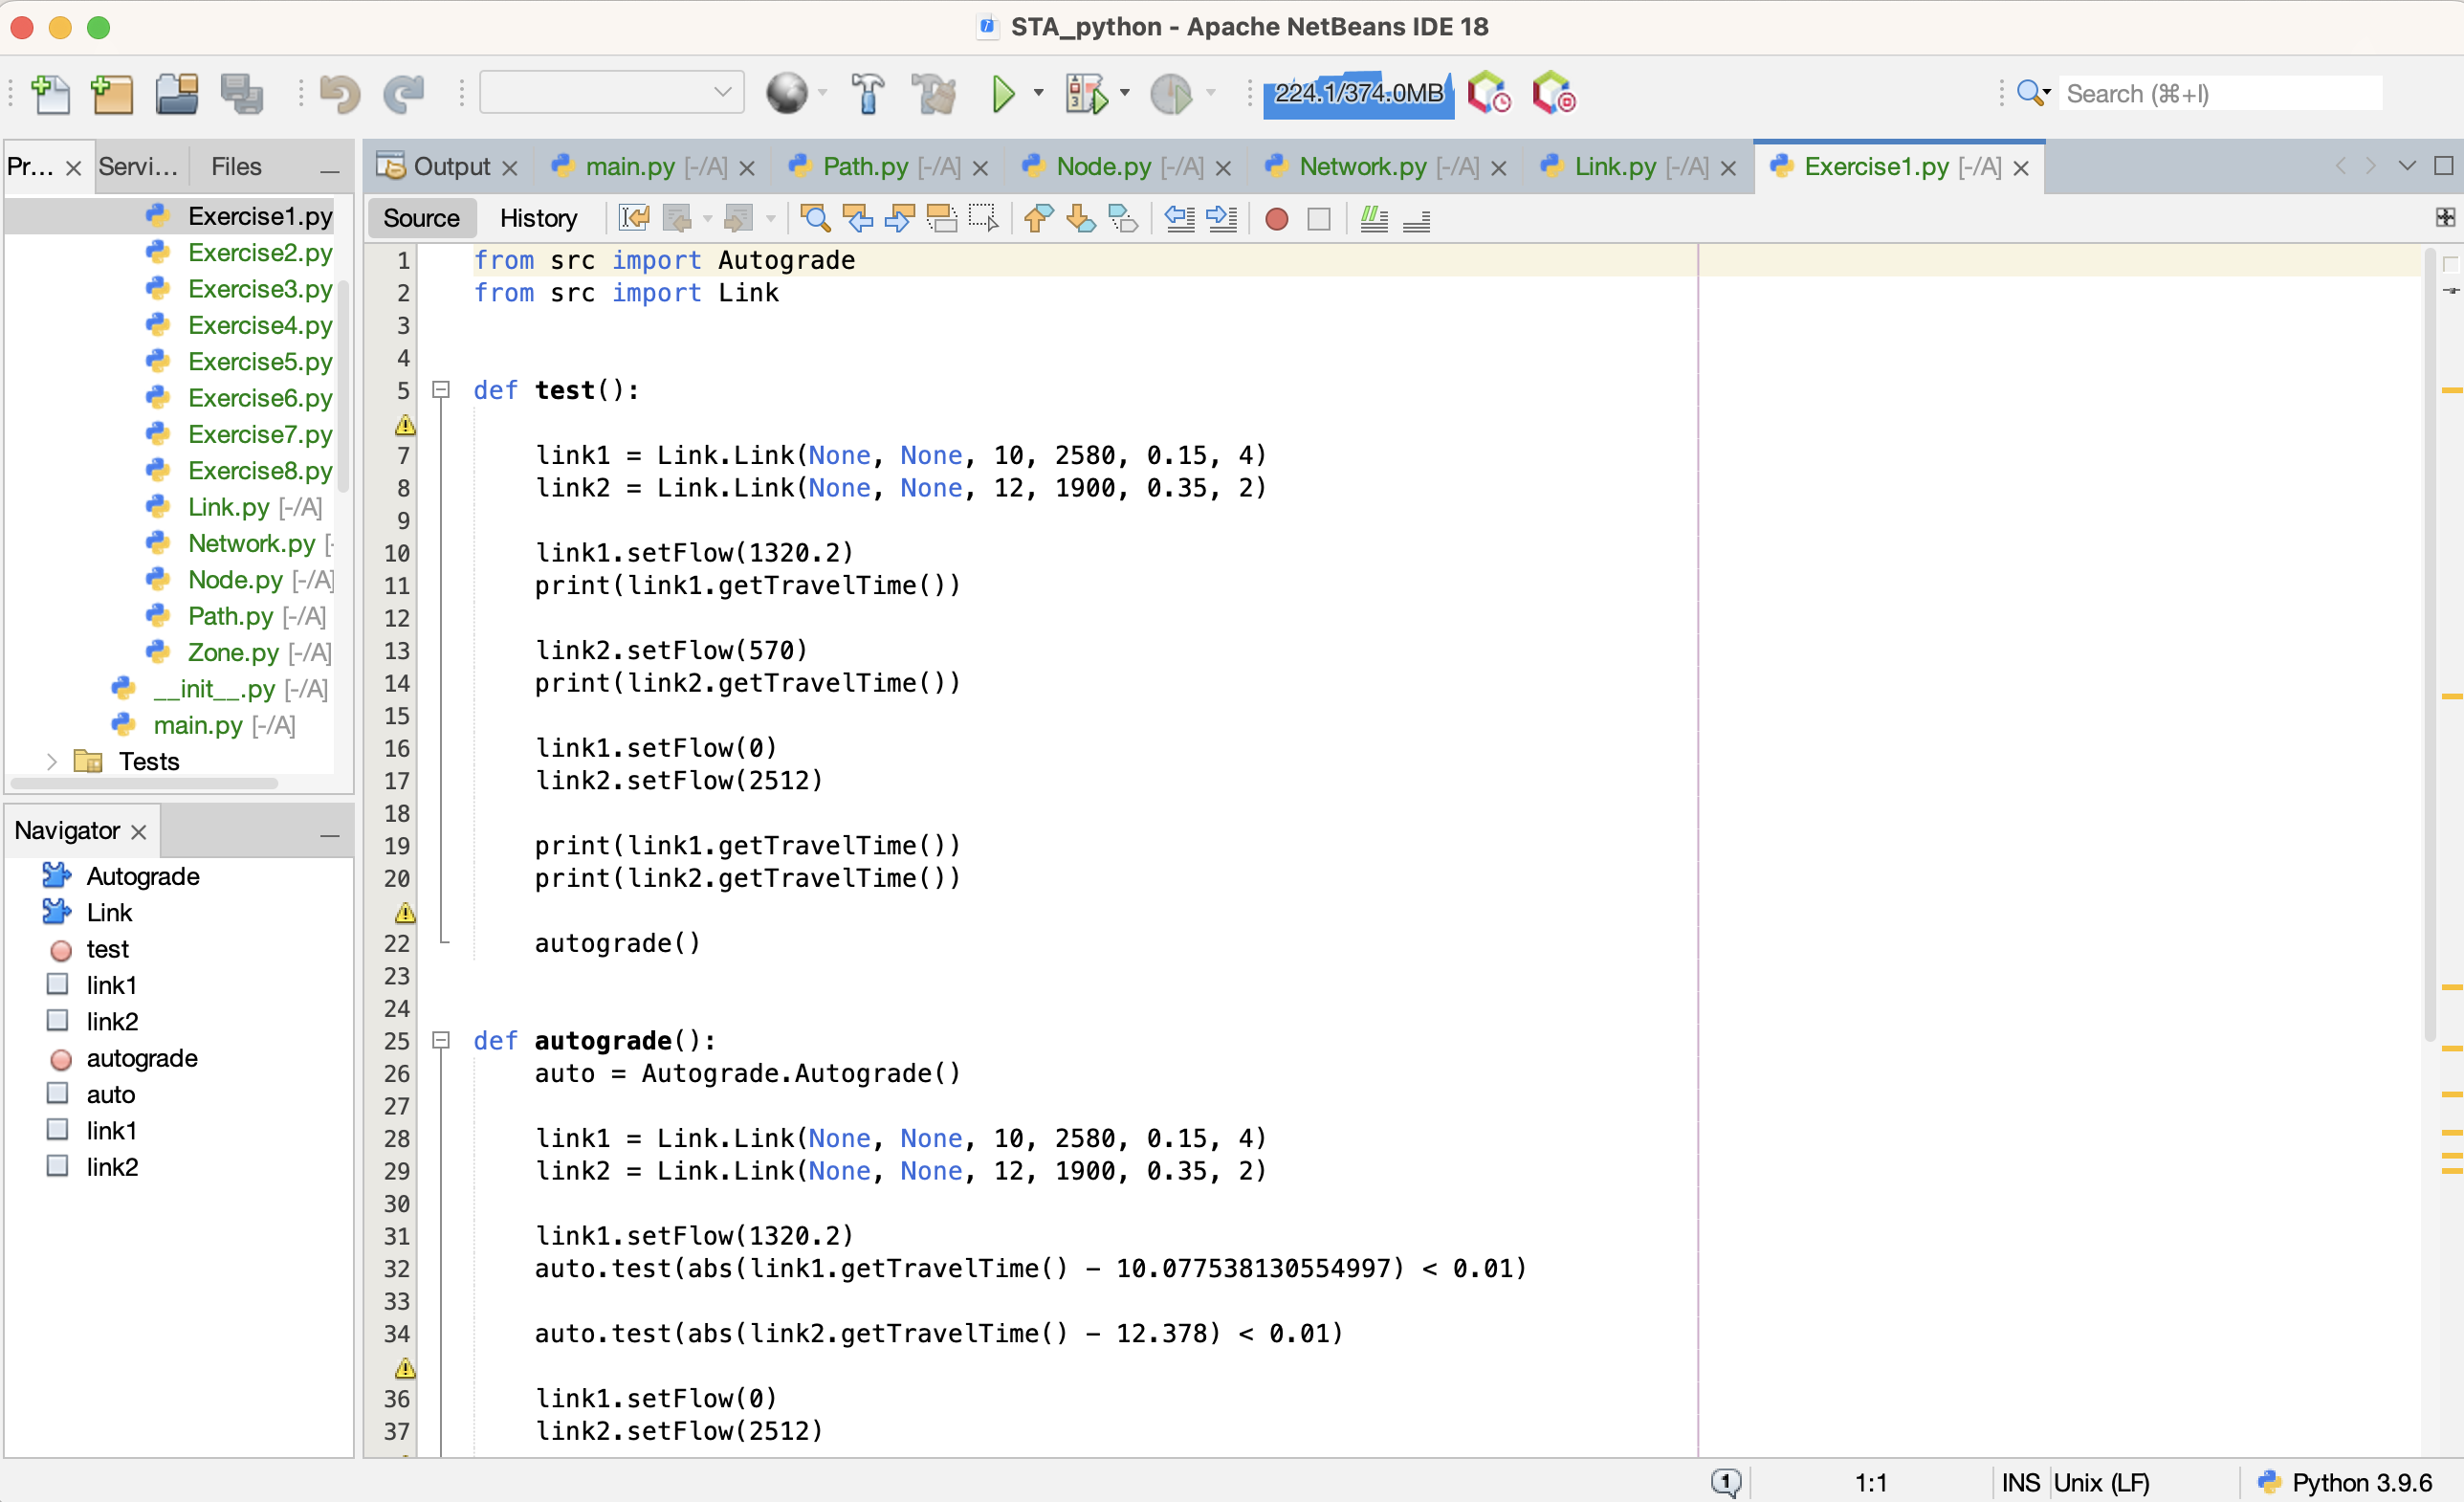
\includegraphics[width=0.5\textwidth]{netbeans4.png}
\end{center}
	
Here is the expected output if the function is implemented correctly:


	\begin{center}
	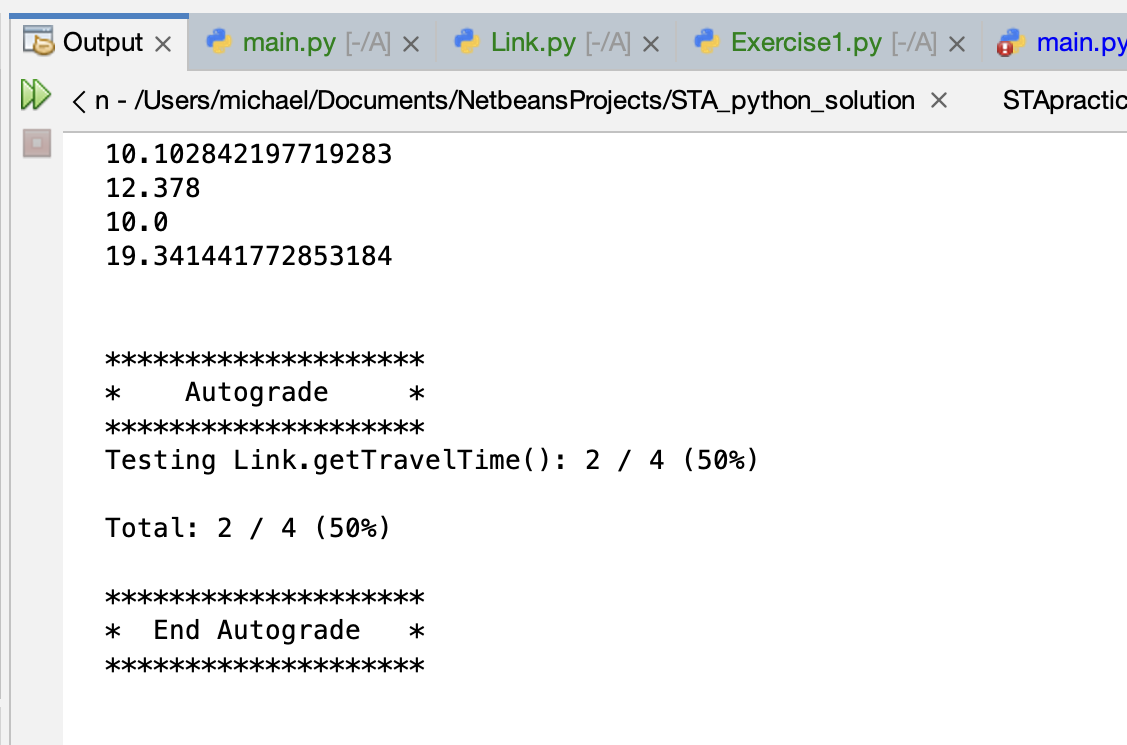
\includegraphics[width=0.5\textwidth]{netbeans5.png}
\end{center}	
	
	
	\paragraph*{A note on testing.} The \texttt{autograde()} functions of each Exercise.py file are merely provided to check correctness. If your code is not correct, they will not indicate what the error is. This is to encourage good testing practice. In the \texttt{test()} function of each Exercise.py file, some code is provided which constructs \texttt{Link}s, \texttt{Node}s, or anything else relevant to the exercise. You can use this space to test the output of the function you wrote for the exercise and compare it to what you calculate by hand to be the correct answer. Once you believe your code is correct, use the \texttt{autograde()} function to verify correctness.
	
	
	
\subsection{Iterating through links}
\label{sec22}	
	
Read the tutorials on \href{https://www.w3schools.com/python/python_functions.asp}{defining functions}.  When working with functions within classes, remember to use the \href{https://www.w3schools.com/python/gloss_python_self.asp}{``\texttt{self}'' reference} to access instance variables.
	
\paragraph*{Exercise 2(a)} Open Link.py. 
Implement the following:
\begin{itemize}
\item \texttt{getFlow()} function: returns the flow of the link

\item \texttt{getCapacity()} function: returns the capacity of the link
\end{itemize}
\textit{Hint:} the link flow is $x_{ij}$ and the link capacity is $C_{ij}$. You already have variables for these values. It is good programming practice to separate the variables from other parts of the code through accessor functions. 

\vspace{\baselineskip}

\noindent
Read the tutorials on \href{https://www.w3schools.com/python/python_booleans.asp}{booleans}. Then, read the tutorial on using \texttt{boolean} values to control the program flow through \href{https://www.w3schools.com/python/python_conditions.asp}{\texttt{if}, \texttt{elif}, and \texttt{else} statements}. 

Now we need to introduce the first data structure, a list. A list is simply an ordered list of elements with a fixed size. Read the \href{https://www.w3schools.com/python/python_lists.asp}{tutorial on lists}. When working with lists, it is helpful to use loops. Read the tutorials on \href{https://www.w3schools.com/python/python_lists_loop.asp}{looping through lists}.
Loops are an essential element of programming. Read the tutorials on \href{https://www.w3schools.com/python/python_for_loops.asp}{for loops} and \href{https://www.w3schools.com/python/python_while_loops.asp}{\texttt{while} loops}, and \href{https://www.w3schools.com/python/ref_keyword_break.asp}{breaking a loop}.

We will be working with strings in the next exercise, so read the \href{https://www.w3schools.com/python/python_strings.asp}{tutorial on strings}.

\paragraph*{Exercise 2(b)} Open Exercise2.py. Your task is to implement the \texttt{findCongestedLinks()} function in Exercise2.py, which outputs a string containing some information about each link.  The list of links is passed as a function parameter. For each link in the list, first add ``link'' to the string and then the index of the link starting at 1, i.e. ``1'', ``2'', etc. Then add the link travel time, and finally add ``yes'' if $x_{ij}/C_{ij} >1$, or ``no'' if $x_{ij}/C_{ij} \leq 1$. After each link, add a newline to the string by adding ``\textbackslash n''. 


You may need to \href{https://www.w3schools.com/python/python_casting.asp}{cast numbers as a string}.


Return the completed string as the output of the \texttt{findCongestedLinks()} function.
	Your output should look something like this:
	\begin{align*}
		& \texttt{link 1 10.171386840006189 yes} \\
		&\texttt{link 2 7.69733539223671 no} \\
		& \ldots
	\end{align*}
	
	 \vspace{\baselineskip}
	
	\noindent
After completing Exercises 2(a) and 2(b), your code should pass the \texttt{autograde()} function of Exercise2.py. 
	
	
	
	
\section{Object-oriented programming}

\subsection{Network structure}

\label{sec31}
	
You have already been working with the \texttt{Link} class to represent links in the network. It is time to learn enough about object-oriented programming to represent the entire network $\mathcal{G}$. Read the tutorial on \href{https://www.w3schools.com/python/python_classes.asp}{classes}. You have already worked with the \texttt{getTravelTime()}, \texttt{getCapacity()}, and \texttt{getFlow()} functions of the \texttt{Link} class. 
Note that when a new instance of a class is created, the constructor function \texttt{\_\_init\_\_()} is automatically invoked. 

When creating a new integer or float variable, you can set the initial value to 0 or 0.0. When creating a new object, e.g. an instance of \texttt{Link}, the default or empty value is \href{https://www.w3schools.com/python/ref_keyword_none.asp}{\texttt{None}}. 
 
 
 \paragraph*{Exercise 3(a)} Open Node.py. You will notice that a \texttt{Node} class has already been created for you.
 
 Open Link.py. Implement the following:
 \begin{itemize}
 	\item \texttt{getStart()} function: returns the start node of the link.
 	\item  \texttt{getEnd()} function: returns the end node of the link.
 \end{itemize} 
 In terms of the model, link $(i,j)$ has start node $i$ and end node $j$. These are already stored as instance variables in the \texttt{Link} class. 

Open Link.py. You will notice that the first function \texttt{\_\_init\_\_()} is a constructor which stores the passed link parameters \texttt{start}, \texttt{end}, \texttt{t\_ff}, \texttt{C}, \texttt{alpha}, and \texttt{beta} in the instance variables. 

\paragraph*{Exercise 3(b)} Open Node.py. Implement the function \texttt{getId()} of the \texttt{Node} class. 
Each node has an id --- an integer that is used to identify the node. Ids start at 1 and increment upwards.  When a node is constructed, the id is passed as a parameter into the constructor for the \texttt{Node class}. The constructor parameter is a single \texttt{int} representing the id of the node. Therefore, the constructor looks like \texttt{\_\_init\_\_(self, id)}.


Also implement the constructor for the \texttt{Node} class. To do so, you may need to add instance variables to the \texttt{Node} class, e.g. an instance variable storing the id of the node.


\paragraph*{Exercise 3(c)}
When you print an instance of a class, it will by default call the \texttt{\_\_str\_\_()} method of that class. Unless you implement it, the output will be a memory reference that is usually not useful.
\begin{itemize}
	 \item Implement the \texttt{\_\_str\_\_()} function of the \texttt{Node} class to return a string containing the id of the node.
	  \item Implement the \texttt{\_\_str\_\_()} function of the \texttt{Link} class to return the string ``($i$, $j$)'' where $i$ and $j$ are the ids of the start and end nodes. For instance, a link from node 1 to node 2 should have a \texttt{\texttt{\_\_str\_\_()}} output of ``\texttt{(1, 2)}''. 
\end{itemize}
% 



\paragraph*{Exercise 3(d)} 
\begin{itemize}
	\item Open Node.py. Implement the \texttt{getOutgoing()} function of the \texttt{Node} class. It returns a list of links that are outgoing from the given node. For node $i$, the list of outgoing links contains all links $(i, j)$ that start at $i$.
	
	\textit{Hint:} you will need to create a new instance variable  in the \texttt{Node} class to store that list of outgoing links $\Gamma^+_i$ --- do so in the constructor of the \texttt{Node} class.
	
	
	\item Implement the \texttt{addOutgoingLink(ij)} function  in the \texttt{Node} class which adds \texttt{Link ij}  to the list that you just created. 
	
	Then call this function in the constructor of the \texttt{Link} class so that every time a \texttt{Link} from $i$ to $j$ is created, it is added to the list of outgoing links of $i$.
\end{itemize}


 \vspace{\baselineskip}

\noindent
After completing Exercises 3(a)--3(d), your code should pass the \texttt{autograde()} method of Exercise3.py. 



% exercise 4: Zone class that stores demand

\subsection{Inheritance}
\label{sec32}

Our next step is to create a representation of the demand $d_{rs}$. To do so, we will create a new \texttt{Zone} class that is a special type of \texttt{Node}: the \texttt{Zone} $r$ stores the demand $d_{rs}$. Read the tutorials on \href{https://www.w3schools.com/python/python_inheritance.asp}{inheritance}. Open Zone.py. 
The \texttt{Zone} class extends the \texttt{Node} class, which is indicated by the definition ``\texttt{class Zone(Node.Node)}''.
 
For the next exercise, we will be implementing the \texttt{getDemand(dest)} function of the \texttt{Zone} class, which returns the demand $d_{rs}$ from node $r$ (the \texttt{Zone} being referenced) to a destination node \texttt{dest}. 

When we read the file, we will store demand in the \texttt{Zone} instance of $r$ by calling the \texttt{addDemand(s, d)} function to add $d$ demand from $r$ to $s$.
To assist in this implementation, learn about \href{https://www.w3schools.com/python/python_dictionaries.asp}{maps}. 
	
	
\paragraph*{Exercise 4(a)} Open Zone.py. Implement the constructor of the \texttt{Zone} class.
You can call methods of the parent class using the \href{https://www.w3schools.com/python/ref_func_super.asp}{\texttt{super()}} function.

\paragraph*{Exercise 4(b)} 
\begin{itemize}
\item Open Zone.py. Implement the \texttt{addDemand(dest, demand)} function of the \texttt{Zone} class. This function is called on zone $r$ to increase $d_{rs}$ for a parameter $s$. This function must store the demand added for later reference by the \texttt{getDemand(dest)} method. 
\item 
Implement the \texttt{getDemand(s)} function, which returns the total demand from $r$ to $s$.

\textit{Hint: } Create a dictionary instance variable in the \texttt{Zone} class to store the demand.
\end{itemize}

\paragraph*{Exercise 4(c)} Open Zone.py. The productions of a zone $P_r$ is defined as $P_r=\sum\limits_{s\in\Z}d_{rs}$. Implement the \texttt{getProductions()} function of the \texttt{Zone} class, which returns the total productions of the zone. \textit{Hint:} Iterate through all stored demand.


\paragraph*{Exercise 4(d)} Some zones are not through nodes, meaning that they can be used as destinations but not as intermediate nodes for travel. The function \texttt{isThruNode()} of class \texttt{Node} returns a boolean indicating whether a \texttt{Node} is a through node. 

In the \texttt{Node} class, the function always returns \texttt{True}. Some \texttt{Zone}s may not be a through node, meaning that the function should return \texttt{False} for them. In a later exercise, we will identify which nodes are through nodes.

Read the tutorial on \href{https://www.w3schools.com/python/python_inheritance.asp}{inheritance} to learn about overloading functions. 
\begin{itemize}
	\item Open Zone.py. Implement the \texttt{setThruNode()} function: it takes a boolean parameter indicating whether this zone is a through node. You will need to store it in an instance variable to implement the next function.
	\item Implement the \texttt{isThruNode()} function. It returns a boolean indicating whether the zone is a through node.
\end{itemize}



 \vspace{\baselineskip}

\noindent
After completing Exercises 4(a)--4(d), your code should pass the \texttt{autograde()} method of Exercise4.java. 
% add through node to Node




% exercise 5: read network

\subsection{Reading network from files}
\label{sec33}


Open Network.py. It contains the \texttt{Network} class, which represents $\mathcal{G}$ in the network definition $\mathcal{G}=(\N, \A)$. Therefore, it stores the nodes and links of the network, and includes some functions for network calculations.
%
It has been partially implemented for you. There are instance variable lists of \texttt{Node}s, \texttt{Link}s, and \texttt{Zone}s, which represent the sets $\N$, $\A$, and $\Z$ of the network. There are also accessor methods for each of these lists. 

The next step is to populate these sets with network data. Thus far, we have been creating specific instances of \texttt{Node}s and \texttt{Link}s in the Exercise.py files. To keep our code more general, we want to keep the problem-specific data in data files rather than in the code. Fortunately, data for many networks is available on \href{https://github.com/bstabler/TransportationNetworks}{Ben Stabler's Github account}. 


Before we discuss the data format, we need to learn how to read from a file. Read the tutorial on  \href{https://www.w3schools.com/python/python_file_open.asp}{reading from a file}. The functions \href{https://www.w3schools.com/python/ref_file_readline.asp}{\texttt{readline()}} and \href{https://www.w3schools.com/python/ref_file_readlines.asp}{\texttt{readlines()}} methods may be useful here also. 

We will need to extract individual numbers from the file. I suggest using the \href{https://www.w3schools.com/python/ref_string_split.asp}{\texttt{split()} function}. Occasionally, when you read a line, you will end up with extra whitespace at the end, e.g. in the string `` extra space ''. You can remove that using the \href{https://www.w3schools.com/python/ref_string_strip.asp}{\texttt{strip()} function}. You may come across a number that is given as a string, e.g. the string ``26.2'', but you want to convert it to integer or float type. Use the \href{https://www.w3schools.com/python/python_casting.asp}{casting functions}. 

In this project, the network data is contained within the folder ``data/[network name]/''. Each network is specified by two text files, ``net.txt'' and ``trips.txt''.  The constructor \texttt{Network(name)} constructs the \texttt{Network} by calling the \texttt{readNetwork(file)} and \texttt{readTrips(file)} functions for the given network name. 
%
The first file, ``net.txt'', defines the links and their characteristics. An example is shown below:

\begin{center}
	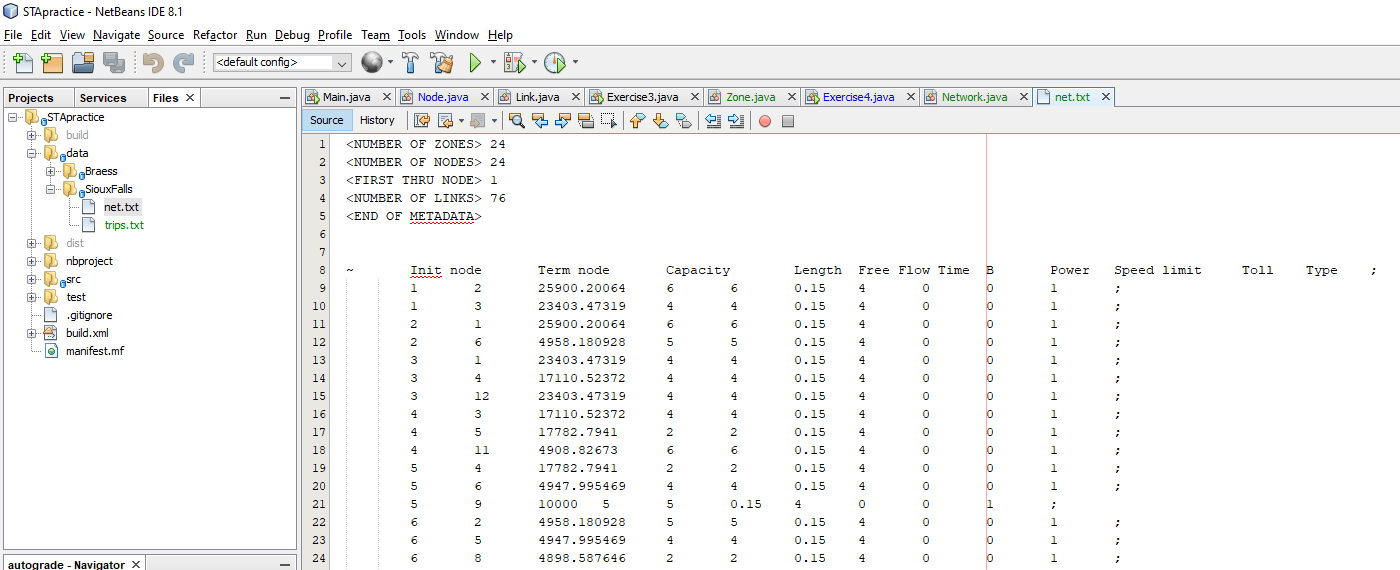
\includegraphics[width=\textwidth]{netbeans6.png}
\end{center}


\noindent The first section contains the metadata, which specifies the size of the sets $\N$, $\A$, and $\Z$. This section is ended by the line ``<END OF METADATA>''. Nodes are labeled by the numbers $1\ldots \vert\N\vert$ where $\vert\N\vert$ is specified in the metadata. 




\paragraph*{Exercise 5(a)} Open Network.py. Add code in the \texttt{readNetwork()} function to read the metadata to obtain the numbers of nodes, zones, and links.

\textit{Hint:} loop until the line \texttt{<END OF METADATA>} is reached. If an intermediate line contains the text \texttt{<NUMBER OF NODES>}, then use that number to instantiate the \texttt{nodes} array. Repeat for the \texttt{links} and \texttt{zones}. 


\paragraph*{Exercise 5(b)} 

 \begin{itemize}
 	\item Open Network.py. Zones are labeled $1$ through $\vert \Z \vert$. Populate the instance variable list \texttt{zones} in the \texttt{Network} class by constructing a new instance of \texttt{Zone} in the  \texttt{readNetwork()} function and store them in the list \texttt{zones}.
 	
 	\textit{Hint:} the number of nodes in the metadata specifies the number of zones to construct.
 	
 	\item Populate the instance variable list \texttt{nodes}  in the \texttt{Network} class Nodes are labeled $1$ through $\vert \N \vert$, which includes some nodes that are also zones. Construct new nodes in the  \texttt{readNetwork()} function and add them to the list \texttt{nodes} as needed. 
 	
 	Do not construct new instances of \texttt{Node} for  zones that you already constructed. Use the instance of \texttt{Zone} that already exists in the array \texttt{zones}. 
 \end{itemize} 


\paragraph*{Exercise 5(c)} After the header line, each line of data contains the parameters for one link in a specific order: start node, end node, capacity, length, free flow time, $\alpha_{ij}$, $\beta_{ij}$, speed limit, toll, and type. ``B'' refers to $\alpha_{ij}$ and ``power'' refers to $\beta_{ij}$. Some of these are not used in this tutorial. 

In the \texttt{readNetwork()} function of the \texttt{Network} class, read the data and use it to construct a new \texttt{Link} instance for each link. Store those instances in the list \texttt{links}.
 \textit{Hint:} the number of links in the metadata specifies the number of lines of data. 


\vspace{\baselineskip}

\noindent
The second file is ``trips.txt''. The metadata here can be ignored. For each zone $r$, the keyword \texttt{Origin} defines the start of the demand array $d_{rs}$ for each zone $s$. That demand is specified over the next several lines.

\begin{center}
	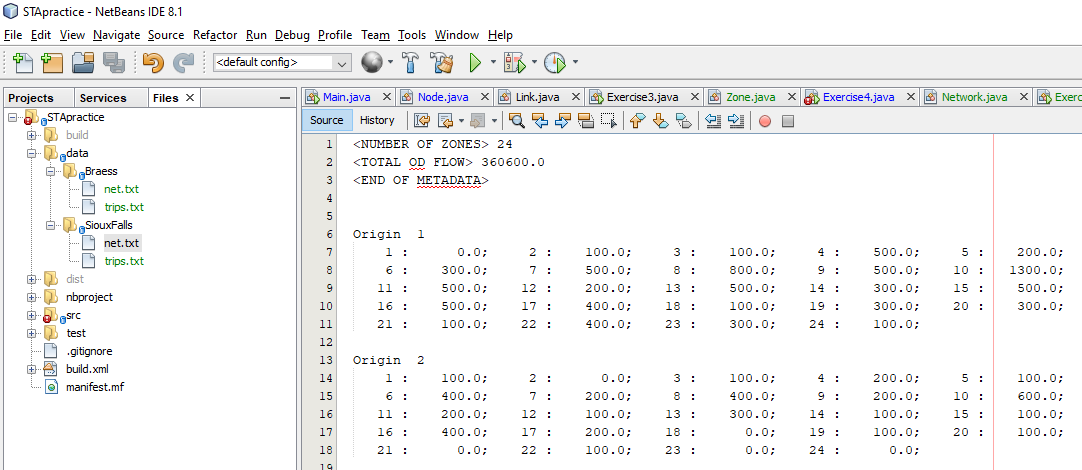
\includegraphics[width=\textwidth]{netbeans7.png}
\end{center}

\paragraph*{Exercise 5(d)} Open Network.py. In the \texttt{readTrips()} function, read the origin-destination trip matrix, and store it in the \texttt{Zone} instances using the \texttt{addDemand()} function of class \texttt{Zone}. 

\textit{Hint:} Iterate through each line to the end of the metadata using a \texttt{while} loop until you reach the text \texttt{<END OF METADATA>}. Then look for origins denoted by the \texttt{Origin} keyword. Then look for destination node ids until you reach the next \texttt{Origin} keyword. Use the \href{https://www.w3schools.com/python/ref_string_split.asp}{\texttt{split()} function} to obtain individual data, e.g. ``Origin'', zone ids, demand numbers, etc.


\paragraph*{Exercise 5(e)} For testing or data analysis, you may find it helpful to find the \texttt{Node} associated with a given id, or the \texttt{Link} between two \texttt{Node}s. 
\begin{itemize}
	\item Open Network.java. Implement the \texttt{findNode()} function, which returns the node with the given id, or \texttt{None} if none exists.
	
	\item Implement the \texttt{findLink()} function, which returns the link between the 2 given nodes, or \texttt{None} if none exists.
\end{itemize}
\textit{Hint:} You have a list of all \texttt{Node}s available in the \texttt{Network} class, and a list of all outgoing links from a given \texttt{Node}. 


 \vspace{\baselineskip}


\noindent
After completing Exercises 5(a)--5(e), your code should pass the \texttt{autograde()} method of Exercise5.py. 




\section{Data structures and algorithms}


\subsection{Dijkstra's algorithm}


We are now ready to implement a shortest path algorithm, which will be used in the method of successive averages. We will implement the well-known Dijkstra's algorithm, which finds the one-to-all shortest path. For more information on Dijkstra's, see \href{https://sboyles.github.io/blubook.html}{\textit{Transportation Network Analysis}}. We need to define two additional variables. Let $c_n\in\mathbb{R}_+$ be the cost label of node $n$, and let $p_n\in\N$ be the predecessor node. First, read through a pseudocode of this algorithm:


\vspace{\baselineskip}


\begin{algorithmic}[1]
	\Procedure{Dijkstra's}{$r$} 
	\For{$n\in \N$} \Comment{Initialization} \label{line1}
	\State $c_n \leftarrow \infty$
	\State $p_n \leftarrow \emptyset$
	\EndFor
	\State $c_r \leftarrow 0$ \label{line6}
	\State  $Q\leftarrow \{r\}$ \label{line7}
	
	\vspace{0.5\baselineskip}
	
	\While{$Q\neq\emptyset$} \Comment{Main loop} \label{line8}
	\State $u\leftarrow \argmin\limits_{n\in Q} \left\{ c_n\right\}$ \label{line9}
	\State $Q\leftarrow Q/\{u\}$
	\For{$(u,v)\in\A$} \label{line10}
	\If{$c_u+t_{uv} < c_v$} \Comment{Is this a shorter path to $v$?} \label{line11}
	\State $c_v \leftarrow c_u + t_{uv}$ \Comment{If so, update $v$ and add it to $Q$} \label{line12}
	\State $p_v \leftarrow u$
	\State $Q\leftarrow Q\cup \{v\}$ \label{line14}
	\EndIf
	\EndFor
	\EndWhile \label{line17}
	\EndProcedure 
	
\end{algorithmic}

\vspace{\baselineskip}

\noindent This may be your first time implementing pseudocode, so we will break it down into steps. The first is the initialization. In line \ref{line1}, we start looping through all nodes in set $\N$. Within this loop, set $c_n \leftarrow \infty$. The operator $\leftarrow$ is used to indicate that $c_n$ is assigned the value $\infty$, which \href{https://www.w3schools.com/python/ref_math_inf.asp}{exists in python}. $p_n$ is assigned the value $\emptyset$, or \texttt{None} in Python, i.e. $p_n$ is initialized to not be any specific node. After the loop, in line \ref{line6} we set $c_r\leftarrow 0$. Recall that $r$ is the origin parameter to Dijkstra's, so $r$ is the starting point. Therefore the shortest path from $r$ to $r$ has cost $0$. Finally, in line \ref{line7} we construct the set $Q\subseteq\N$ which contains the unsettled nodes. 

Next, we enter the main loop in line \ref{line8}. This loop continues while $Q$ is non-empty --- while there is an unsettled node that we need to visit. Line \ref{line9} is written very simply, but can actually require more extensive code. Finding the $\argmin_{n\in Q} \left\{c_n\right\}$ could involve looping through all elements of $Q$ to find the $n$ with the smallest value of $c_n$. Save that node and store it in variable $u$. Once you have determined $u$, remove it from $Q$. Then loop through all outgoing links $(u,v)$ in line \ref{line10}. The function \texttt{getOutgoing()} of the \texttt{Node} class which you implemented previously will be useful here. In line \ref{line11}, notice that while $c_u$ and $c_v$ will be variables, $t_{uv}$ is a function call to \texttt{getTravelTime()} of the \texttt{Link} class. Line \ref{line14} requires adding node $u$ to set $Q$. Beware of adding multiple copies of $u$ to your implementation of $Q$, which is possible with some data structures (such as lists). Instead, use a \href{https://www.w3schools.com/python/python_sets.asp}{python set} to implement the set $Q$. If done correctly, $Q$ will eventually become empty, and the algorithm will terminate after calculating $c_n$ and $p_n$ for all nodes. 






We will start our implementation of Dijkstra's by implementing a data structure to store a path. 
A \texttt{Path} is an ordered list of \texttt{Link}s. Open Path.py. A \texttt{Path} contains a list of links and includes the following functions:
\begin{itemize}
	\item \texttt{add()}: add a link to the end of the list.
	\item \texttt{addFront()}: add a link to the front of the list.
	\item \texttt{size()}: returns the size of the list.
\end{itemize}

In addition, \texttt{Path} defines five additional functions to perform calculations on the path:
\begin{itemize}
	\item \texttt{isConnected()} checks whether the list of links is a valid path. For instance, the list \texttt{[(1,3), (3, 7), (7, 8)]} is a connected path, but the list \texttt{[(1,3), (2, 4), (4, 8)]} is not.
	\item  \texttt{getSource()} and \texttt{getDest()} return the origin and destination nodes of the path, respectively.
	\item \texttt{getTravelTime()} calculates $T^\pi$.
	\item \texttt{addHstar()} will be used later.
\end{itemize}


\paragraph*{Exercise 6(a)} 
\begin{itemize}
	\item Open Path.py. Implement the \texttt{getSource()} function: return the starting node of the path.
	
	\textit{Hint.} You have a list of all links in the path.
	
	\item Implement the \texttt{getDest()} function: return the last node of the path.
	\item Implement the \texttt{isConnected()} function, which checks whether the list of links is a connected path.
	\item Implement the \texttt{getTravelTime()} function, which returns $T^\pi = \sum_{(i,j)\in\pi} t_{ij}(x_{ij})$.
\end{itemize}



\vspace{\baselineskip}

\noindent
To implement Dijkstra's, we need two additional variables $c_n$ and $p_n$.
Open Node.py. You will see that the instance variables \texttt{cost} (representing $c_n$) and \texttt{predecessor} (representing $p_n$) have already been created for you.

% 6b dijkstra's initialization

\paragraph*{Exercise 6(b)} Open Network.py and navigate to the \texttt{dijkstras()} function. Implement the initialization (lines \ref{line1}--\ref{line7}) of Dijkstra's algorithm. 
You may wish to test the correctness of the initialization before proceeding further. 


% 6c dijkstra's main loop
\paragraph*{Exercise 6(c)} In Network.py, implement the main loop of Dijkstra's algorithm (lines \ref{line8}--\ref{line17}) in the \texttt{dijkstras()} function. 

\vspace{\baselineskip}

\noindent
After executing Dijkstra's algorithm, we now have all the information needed to find the shortest path from $r$ to $s$ through the predecessor labels. We need to convert those predecessor labels into an instance of the \texttt{Path} class created earlier. This can be accomplished through the trace algorithm shown below. Essentially, start at $s$, and follow the predecessor labels until reaching $r$, adding each link to the path as you go. 

\vspace{\baselineskip}

\begin{algorithmic}[1]
	\Procedure{trace}{$r, s$}
	\State $n\leftarrow s$
	\State $\pi \leftarrow \emptyset$
	
	\vspace{0.5\baselineskip}
	
	\While{$n\neq r$}
	\State $\pi\leftarrow \pi \cup \{(p_n,n)\}$
	\State $n\leftarrow p_n$
	\EndWhile
	\EndProcedure
\end{algorithmic}

%\vspace{\baselineskip}

\paragraph*{Exercise 6(d)} Open Network.py. Implement the \texttt{trace()} function in the \texttt{Network} class. 
Remember to add the links in the correct order to ensure a connected path, which can be checked afterwards by the \texttt{isConnected()} function of the \texttt{Path} class.

 \vspace{\baselineskip}


\noindent
After completing Exercises 6(a)--6(d), your code should pass the \texttt{autograde()} method of Exercise6.py. 


\subsection{Network statistics}

Before implementing the method of successive averages, there are some network statistics that will be used in the implementation. These are the total system travel time, $TSTT$, the shortest path travel time, $SPTT$, and the average excess cost, $AEC$. These are defined mathematically as follows:
\begin{align}
	TSTT &= \sum\limits_{(i,j)\in\A} x_{ij} t_{ij}(x_{ij})\\
	SPTT &= \sum\limits_{(r,s)\in\Z^2} \mu_{rs} d_{rs}\\
	AEC &= \frac{TSTT- SPTT}{\sum\limits_{(r,s)\in\Z^2} d_{rs}}
\end{align}

\paragraph*{Exercise 7} 
\begin{itemize}
	\item Open Network.py. Implement the \texttt{getTSTT()} function: return the total system travel time.
	\item Implement the \texttt{getSPTT()} function: return the total system travel time if all demand is on the shortest path. 
	
	\item Implement the \texttt{getAEC()} function: return the average excess cost. 
\end{itemize}
After completing them, your code should pass the \texttt{autograde()} function of Exercise7.py. 



\subsection{Method of successive averages}


The method of successive averages is a simple algorithm for solving user equilibrium. Each iteration, it constructs an all-or-nothing flow assignment $\mathbf{x}^\star$ formed by assigning all flow from $r$ to $s$ to the shortest path from $r$ to $s$. Then, it takes a weighted average between the current and the all-or-nothing flow assignment. The weight, or step size, is denoted by $\lambda$. 
This step is repeated until the maximum number of iterations, $I$, is reached. We can track the convergence towards user equilibrium by printing the average excess cost each iteration.
The algorithm is specified below in pseudocode:

\vspace{\baselineskip}

\begin{algorithmic}[1]
	\Procedure{Method of successive averages}{$I$}
	\For{$(i,j)\in\A$} \Comment{Initialization}
	\State $x^\star_{ij} \leftarrow 0$
	\EndFor
	
	\vspace{0.5\baselineskip}
	
	\For{$iteration\leftarrow 1$ to $I$} \label{msa5}
	\For{$r\in\Z$}  \label{msa6}
	\State {\sc Dijkstra's}($r$) \Comment{Find shortest paths from $r$ to $s$}
	\For{$s\in\Z$}
	\State $\pi^\star_{rs} \leftarrow$ {\sc trace($r$, $s$)}
	\For{$(i,j)\in\pi^\star_{rs}$} \Comment{Update all-or-nothing flow assignment}
	\State $x^\star_{ij} \leftarrow x^\star_{ij} + d_{rs}$ \label{msa11}
	\EndFor
	\EndFor
	\EndFor \label{msa14}
	
	\vspace{0.5\baselineskip}
	
	
	\State $\lambda \leftarrow \frac{1}{iteration}$ \Comment{Calculate step size} \label{msa15}
	
	\vspace{0.5\baselineskip}
	
	\For{$(i,j)\in\A$} \Comment{Take weighted average between $\mathbf{x}$ and $\mathbf{x}^\star$} \label{msa16}
	\State $x_{ij} \leftarrow (1-\lambda)x_{ij} + \lambda x^\star_{ij}$ \label{msa17}
	\State $x^\star_{ij}\leftarrow 0$ \label{msa18}
	\EndFor
	
	\vspace{0.5\baselineskip}
	
	\State {\sc Print}($AEC$) \Comment{Track convergence}
	
	\EndFor
	\EndProcedure
\end{algorithmic}

% x star variable, addxstar method, and addFlow() method

\paragraph*{Exercise 8(a)} 
\begin{itemize}
	\item Open Link.py. Create a new instance variable to store $x^\star_{ij}$ in the \texttt{Link} class.
\item In the \texttt{Link} class, implement the \texttt{addXstar()} function which adds the specified flow to the $x^\star_{ij}$ variable.
It will be used to implement line \ref{msa11}. 

\item In the \texttt{Path} class, implement the \texttt{addHstar()} function which adds the specified flow to the $x^\star_{ij}$ variable of every link in the path. Use the \texttt{addXstar()} method of the \texttt{Link} class in your implementation.
\end{itemize}



\paragraph*{Exercise 8(b)} 
\begin{itemize}
	\item Open Network.py. In the \texttt{Network} class, implement the \texttt{calculateStepsize()} function, which determines the value of $\lambda$ in line \ref{msa15}. 
	
	\item Open Link.py. Using this $\lambda$, in the \texttt{Link} class implement the \texttt{calculateNewX()} function, which takes as input $\lambda$ and implements lines \ref{msa17} and \ref{msa18}. 
	
	\item Open Network.py again, and implement the \texttt{calculateNewX()} function of the \texttt{Network} class, which implements the loop in line \ref{msa16}. 
\end{itemize}



\paragraph*{Exercise 8(c)} Open Network.py. Implement the \texttt{calculateAON()} function in the \texttt{Network} class, which is the loop in lines \ref{msa6}--\ref{msa14}. 

\paragraph*{Exercise 8(d)} In the method \texttt{msa(int)} of the \texttt{Network} class, implement the main loop (line \ref{msa5} of the method of successive averages. Most of the work is already done through the previous exercises --- \texttt{Network.calculateAON()},  \texttt{Network.calculateStepSize()}, \texttt{Link.calculateNewX()}, etc. 

The output is a string containing the following: for each iteration, include a row with the iteration number and the average excess cost, as shown below:

\begin{center}
	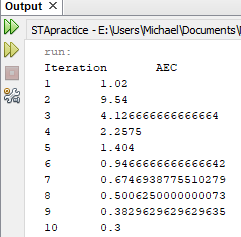
\includegraphics[width=0.3\textwidth]{netbeans8.png}
\end{center}


% calculate step size and update(step size)


% calculate AON


% MSA


	

	
	\noindent
	After completing Exercises 8(a)--8(d), your code should pass the \texttt{autograde()} method of Exercise8.java. 
	
	
	
	
	
	\section{Next steps}
	
	This is not the most efficient implementation of the method of successive averages. Now that you have a correct implementation, you may want to go back and improve the computational efficiency. In addition, the method of successive averages is far from the most efficient algorithm. The Frank-Wolfe algorithm can be implemented in this code fairly easily. You may also wish to try implementing gradient projection~\citep{jayakrishnan1994faster} or Algorithm B~\citep{dial2006path}.
	
	
	
	
	
	
	\bibliography{MWL}
	\bibliographystyle{abbrvnat}
	
	
	
\end{document}